\documentclass[tikz,border=10pt]{standalone}
\usepackage{tikz}
\usetikzlibrary{decorations.pathmorphing}
\input{Core Tikz Library/colours}

\begin{document}

% Q2 (a)(i)
\begin{tikzpicture}
    % Draw the rectangle for the universal set
    \draw[thick] (-2,-2) rectangle (4,2);
    
    % Draw the circles
    \draw[thick] (0,0) circle (1.5cm) node at (-1.8, 1.8) {\(A\)};
    \draw[thick] (2,0) circle (1.5cm) node at (3.8, 1.8) {\(B\)};
    
    % Shade the intersection
    \begin{scope}
        \clip (0,0) circle (1.5cm);
        \fill[primaryBlue, opacity=0.5] (2,0) circle (1.5cm);
    \end{scope}
\end{tikzpicture}

% Q2 (a)(ii)
\begin{tikzpicture}
    % Draw the rectangle for the universal set
    \draw[thick] (-2,-2) rectangle (4,2);
    
    % Draw the circles
    \draw[thick] (0,0) circle (1.5cm) node at (-1.8, 1.8) {\(A\)};
    \draw[thick] (2,0) circle (1.5cm) node at (3.8, 1.8) {\(B\)};
    
    % Shade A ∩ B'
    \begin{scope}
        \clip (-2,-2) rectangle (4,2);
        \fill[primaryBlue, opacity=0.5] (0,0) circle (1.5cm);
        \fill[white] (2,0) circle (1.5cm);
    \end{scope}
    \draw[thick] (0,0) circle (1.5cm);
    \draw[thick] (2,0) circle (1.5cm);
\end{tikzpicture}

% Q2 (a)(iii)
\begin{tikzpicture}
    % Draw the rectangle for the universal set
    \draw[thick] (-2,-2) rectangle (4,2);
    
    % Draw the circles
    \draw[thick] (0,0) circle (1.5cm) node at (-1.8, 1.8) {\(A\)};
    \draw[thick] (2,0) circle (1.5cm) node at (3.8, 1.8) {\(B\)};
    
    % Shade A' ∩ B
    \begin{scope}
        \clip (-2,-2) rectangle (4,2);
        \fill[primaryBlue, opacity=0.5] (2,0) circle (1.5cm);
        \fill[white] (0,0) circle (1.5cm);
    \end{scope}
    \draw[thick] (0,0) circle (1.5cm);
    \draw[thick] (2,0) circle (1.5cm);
\end{tikzpicture}

% Q2 (a)(iv)
\begin{tikzpicture}
    % Draw the rectangle for the universal set
    \draw[thick] (-2,-2) rectangle (4,2);
    
    % Draw the circles
    \draw[thick] (0,0) circle (1.5cm) node at (-1.8, 1.8) {\(A\)};
    \draw[thick] (2,0) circle (1.5cm) node at (3.8, 1.8) {\(B\)};
    
    % Shade A' ∩ B'
    \begin{scope}
        \clip (-2,-2) rectangle (4,2);
        \fill[primaryBlue, opacity=0.5] (-2,-2) rectangle (4,2);
        \fill[white] (0,0) circle (1.5cm);
        \fill[white] (2,0) circle (1.5cm);
    \end{scope}
    \draw[thick] (0,0) circle (1.5cm);
    \draw[thick] (2,0) circle (1.5cm);
\end{tikzpicture}

% Q2 (b)(i)
\begin{tikzpicture}
    % Draw the rectangle for the universal set
    \draw[thick] (-2,-2) rectangle (4,2);
    
    % Draw the circles
    \draw[thick] (0,0) circle (1.5cm) node at (-1.8, 1.8) {\(A\)};
    \draw[thick] (2,0) circle (1.5cm) node at (3.8, 1.8) {\(B\)};
    
    % Shade the union
    \begin{scope}
        \clip (-2,-2) rectangle (4,2);
        \fill[primaryBlue, opacity=0.5] (0,0) circle (1.5cm);
        \fill[primaryBlue, opacity=0.5] (2,0) circle (1.5cm);
    \end{scope}
    \draw[thick] (0,0) circle (1.5cm);
    \draw[thick] (2,0) circle (1.5cm);
\end{tikzpicture}


% Q2 (b)(ii) 
\begin{tikzpicture}
    % Draw the rectangle for the universal set
    \draw[thick] (-2,-2) rectangle (4,2);
    
    % Draw the circles
    \draw[thick] (0,0) circle (1.5cm) node at (-1.8, 1.8) {\(A\)};
    \draw[thick] (2,0) circle (1.5cm) node at (3.8, 1.8) {\(B\)};
    
    % Shade A ∪ B'
    \begin{scope}
        \clip (-2,-2) rectangle (4,2);
        \fill[primaryBlue, opacity=0.5] (-2,-2) rectangle (4,2);
    \end{scope}
    \begin{scope}
        \clip (2,0) circle (1.5cm);
        \fill[white] (-2,-2) rectangle (4,2);
    \end{scope}
    \fill[primaryBlue, opacity=0.5] (0,0) circle (1.5cm);
    \draw[thick] (0,0) circle (1.5cm);
    \draw[thick] (2,0) circle (1.5cm);
\end{tikzpicture}


% Q2 (b)(iii)
\begin{tikzpicture}
    % Draw the rectangle for the universal set
    \draw[thick] (-2,-2) rectangle (4,2);
    
    % Draw the circles
    \draw[thick] (0,0) circle (1.5cm) node at (-1.8, 1.8) {\(A\)};
    \draw[thick] (2,0) circle (1.5cm) node at (3.8, 1.8) {\(B\)};
    
    % Shade A' ∪ B
    \begin{scope}
        \clip (-2,-2) rectangle (4,2);
        \fill[primaryBlue, opacity=0.5] (-2,-2) rectangle (4,2);
    \end{scope}
    \begin{scope}
        \clip (0,0) circle (1.5cm);
        \fill[white] (-2,-2) rectangle (4,2);
    \end{scope}
    \fill[primaryBlue, opacity=0.5] (2,0) circle (1.5cm);
    \draw[thick] (0,0) circle (1.5cm);
    \draw[thick] (2,0) circle (1.5cm);
\end{tikzpicture}



% Q2 (b)(iv)
\begin{tikzpicture}
    % Draw the rectangle for the universal set
    \draw[thick] (-2,-2) rectangle (4,2);
    
    % Draw the circles
    \draw[thick] (0,0) circle (1.5cm) node at (-1.8, 1.8) {\(A\)};
    \draw[thick] (2,0) circle (1.5cm) node at (3.8, 1.8) {\(B\)};
    
    % Shade A' ∪ B'
    \begin{scope}
        \clip (-2,-2) rectangle (4,2);
        \fill[primaryBlue, opacity=0.5] (-2,-2) rectangle (4,2);
        \fill[white] (0,0) circle (1.5cm);
        \fill[white] (2,0) circle (1.5cm);
    \end{scope}
    \draw[thick] (0,0) circle (1.5cm);
    \draw[thick] (2,0) circle (1.5cm);
\end{tikzpicture}

% Q3 
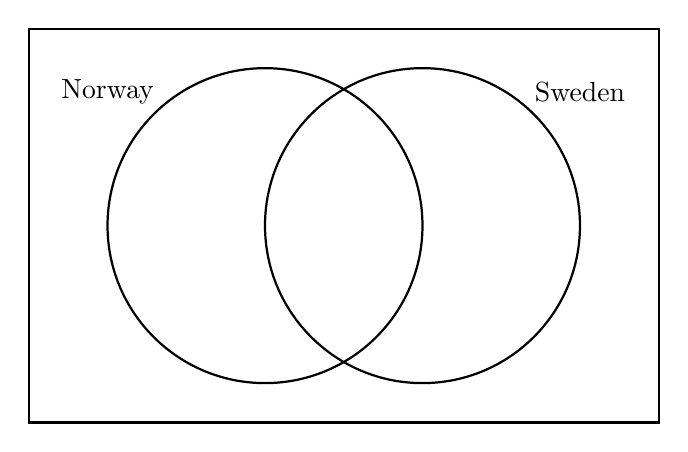
\begin{tikzpicture}
    % Draw the rectangle for the universal set
    \draw[thick] (0,0) rectangle (8,5);

    % Draw the circles
    \draw[thick] (3,2.5) circle (2cm) node at (1, 4.2) {Norway};
    \draw[thick] (5,2.5) circle (2cm) node at (7, 4.2) {Sweden};
    
\end{tikzpicture}

% Q3 - Answer
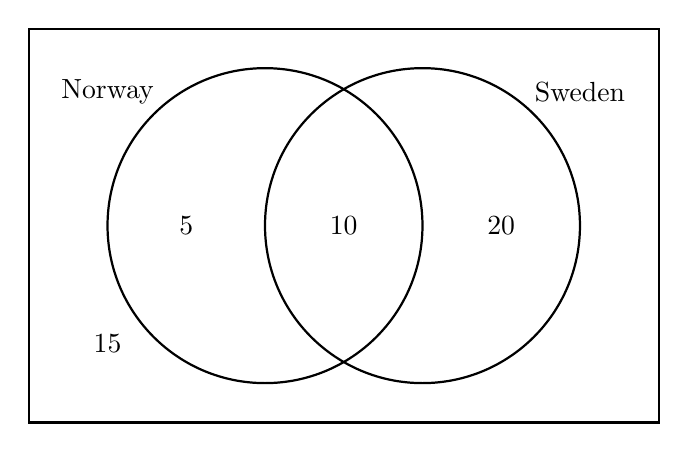
\begin{tikzpicture}
    % Draw the rectangle for the universal set
    \draw[thick] (0,0) rectangle (8,5);

    % Draw the circles
    \draw[thick] (3,2.5) circle (2cm) node at (1, 4.2) {Norway};
    \draw[thick] (5,2.5) circle (2cm) node at (7, 4.2) {Sweden};

    % Numbered entries
    \node at (4,2.5) {10};
    \node at (2,2.5) {5};
    \node at (6,2.5) {20};
    \node at (1,1) {15};
    
\end{tikzpicture}

% Q4
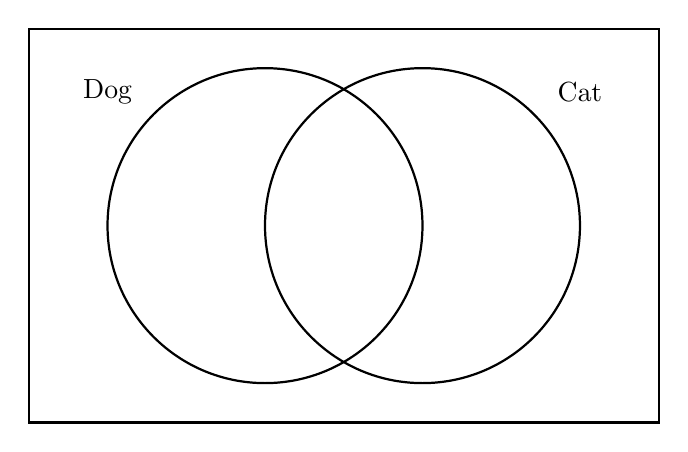
\begin{tikzpicture}
    % Draw the rectangle for the universal set
    \draw[thick] (0,0) rectangle (8,5);

    % Draw the circles
    \draw[thick] (3,2.5) circle (2cm) node at (1, 4.2) {Dog};
    \draw[thick] (5,2.5) circle (2cm) node at (7, 4.2) {Cat};
    
\end{tikzpicture}

% Q4 - Answer
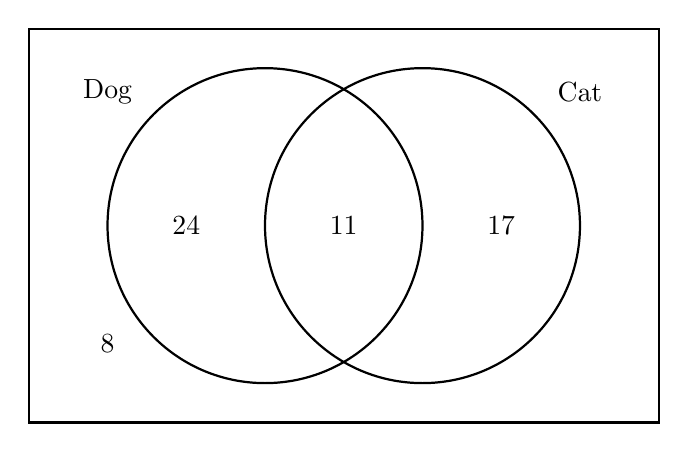
\begin{tikzpicture}
    % Draw the rectangle for the universal set
    \draw[thick] (0,0) rectangle (8,5);

    % Draw the circles
    \draw[thick] (3,2.5) circle (2cm) node at (1, 4.2) {Dog};
    \draw[thick] (5,2.5) circle (2cm) node at (7, 4.2) {Cat};

    % Numbered entries
    \node at (4,2.5) {11};
    \node at (2,2.5) {24};
    \node at (6,2.5) {17};
    \node at (1,1) {8};
    
\end{tikzpicture}

% Q5
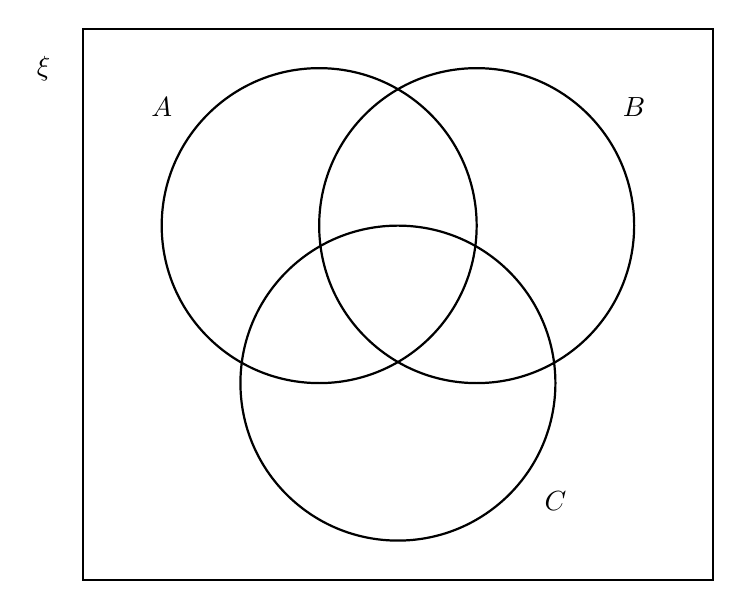
\begin{tikzpicture}
    % Draw the rectangle for the universal set
    \draw[thick] (0,-2) rectangle (8,5);
    
    % Label the universal set
    \node at (-0.5,4.5) {\(\xi\)};

    % Draw the circles
    \draw[thick] (3,2.5) circle (2cm) node at (1, 4) {\(A\)};
    \draw[thick] (5,2.5) circle (2cm) node at (7, 4) {\(B\)};
    \draw[thick] (4,0.5) circle (2cm) node at (6, -1) {\(C\)};
    
\end{tikzpicture}

% Q5 - Answer
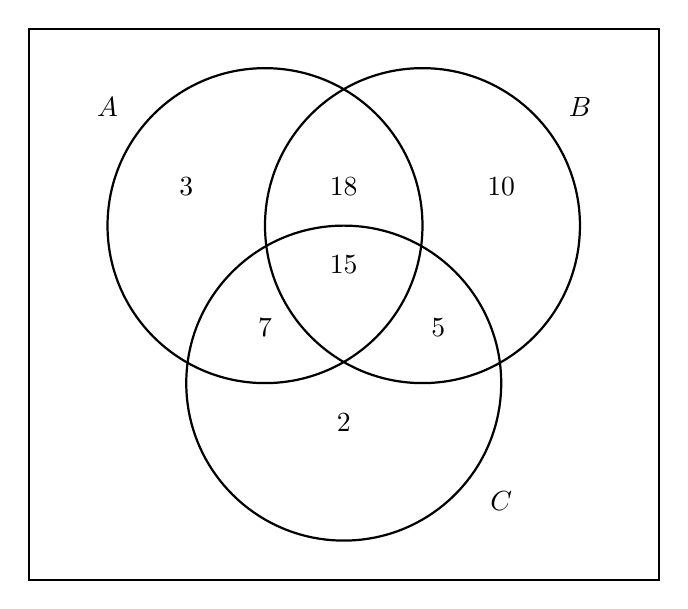
\begin{tikzpicture}
    % Draw the rectangle for the universal set
    \draw[thick] (0,-2) rectangle (8,5);

    % Draw the circles
    \draw[thick] (3,2.5) circle (2cm) node at (1, 4) {\(A\)};
    \draw[thick] (5,2.5) circle (2cm) node at (7, 4) {\(B\)};
    \draw[thick] (4,0.5) circle (2cm) node at (6, -1) {\(C\)};

    % Numbered entries
    \node at (4,2) {15};
    \node at (4,3) {18};
    \node at (5.2,1.2) {5};
    \node at (3,1.2) {7};
    \node at (6,3) {10};
    \node at (4,0) {2};
    \node at (2,3) {3};
    
\end{tikzpicture}

% Q6
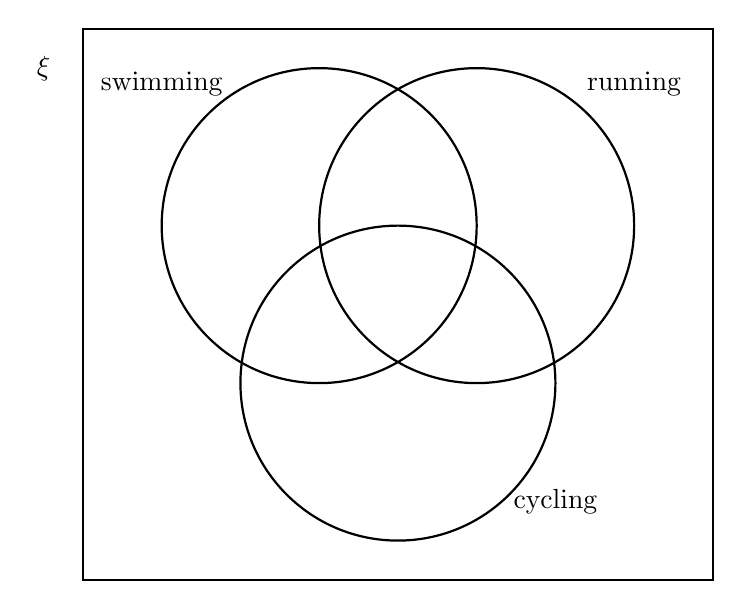
\begin{tikzpicture}
    % Draw the rectangle for the universal set
    \draw[thick] (0,-2) rectangle (8,5);
    
    % Label the universal set
    \node at (-0.5,4.5) {\(\xi\)};

    % Draw the circles
    \draw[thick] (3,2.5) circle (2cm) node at (1, 4.3) {swimming};
    \draw[thick] (5,2.5) circle (2cm) node at (7, 4.3) {running};
    \draw[thick] (4,0.5) circle (2cm) node at (6, -1) {cycling};
    
\end{tikzpicture}

% Q6 - Answer
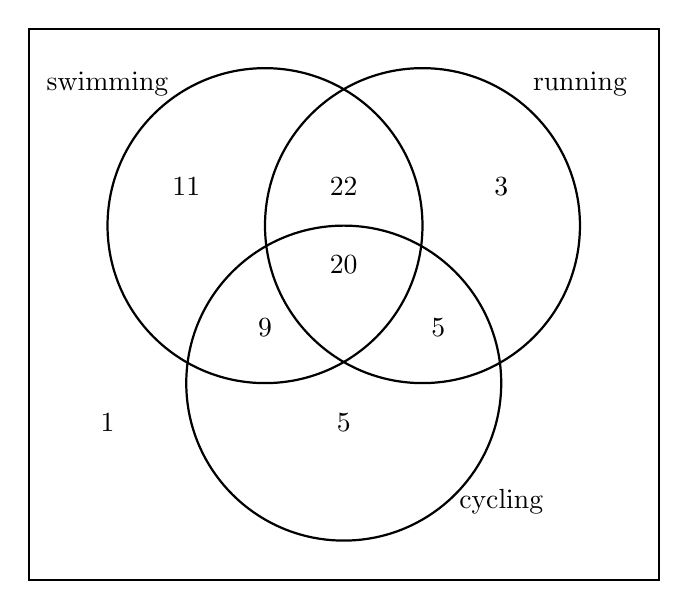
\begin{tikzpicture}
    % Draw the rectangle for the universal set
    \draw[thick] (0,-2) rectangle (8,5);

    % Draw the circles
    \draw[thick] (3,2.5) circle (2cm) node at (1, 4.3) {swimming};
    \draw[thick] (5,2.5) circle (2cm) node at (7, 4.3) {running};
    \draw[thick] (4,0.5) circle (2cm) node at (6, -1) {cycling};

    % Numbered entries
    \node at (4,2) {20};
    \node at (4,3) {22};
    \node at (5.2,1.2) {5};
    \node at (3,1.2) {9};
    \node at (6,3) {3};
    \node at (4,0) {5};
    \node at (2,3) {11};
    \node at (1,0) {1};
    
\end{tikzpicture}

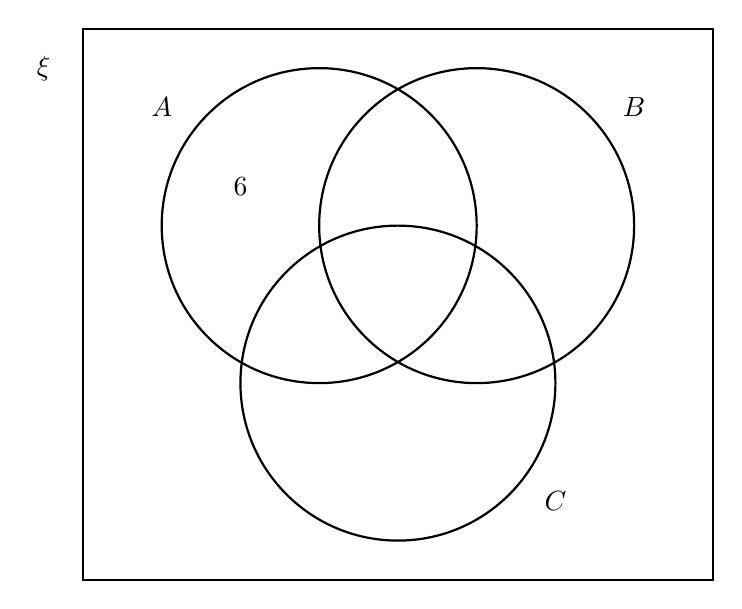
\begin{tikzpicture}
    % Draw the rectangle for the universal set
    \draw[thick] (0,-2) rectangle (8,5);
    
    % Label the universal set
    \node at (-0.5,4.5) {\(\xi\)};

    % Draw the circles
    \draw[thick] (3,2.5) circle (2cm) node at (1, 4) {\(A\)};
    \draw[thick] (5,2.5) circle (2cm) node at (7, 4) {\(B\)};
    \draw[thick] (4,0.5) circle (2cm) node at (6, -1) {\(C\)};
    
    % Numbered entries
    \node at (2,3) {6};
    
\end{tikzpicture}

\end{document}
